\chapter{Transport mode application to heavy-flavor evolution}
In this chapter, we shall start to focus on applying the LIDO transport model to the heavy-flavor section, and discuss in detail how a transport model fits into the complex dynamics that heavy flavor particles undergoes in the heavy-ion collision environment.

Heavy flavor is a charming probe for the medium created in heavy-ion collisions. 
Its large mass guarantees an negligible thermal production contribution at least for present LHC top beam energies for heavy-ion program (there are estimates that thermal contribution can play a row in future FCC collider).
Therefore, heavy flavors are almost always created in initial hard processes. 
By hard processes, it includes both the hardest few body collisions, as well as the associated high-virtuality parton evolution.
Their dilute population also suppresses the chances that they annihilates against their anti-particles during the medium evolution.
As a result, heavy flavors are created at relatively early stages of the heavy-ion collision and experienced the entire medium evolution and encodes valuable information about the medium.
On the theory side heavy flavor has a rich variety of physics interests. 
At high $p_T$, the evolution of heavy flavor particles merges into the context of jet dynamics and jet energy loss study; at intermediate $p_T$ the mass hierarchy predicted for the medium modifications;
and low $p_T$, heavy flavor is one of the key messengers for the thermalization processes inside QGP due to its long relaxation time compared to light partons.
On the experimental side, their unique flavors, masses, and decay modes also give us the chance to reconstruct heavy flavor (heavy meson / baryon) observables directly.

There are two types of heavy quarks that are most relevant for nowadays hard-probes study, the charm quark with mass $1.3$ GeV, and the bottom quark with mass $4.2$ GeV.
The reason top quark ($173$ GeV) is out of our discussion is due to its extremely short life time ($\sim 5\times 10^{-25} \approx 0.15$  fm/$c$ in the rest frame) so it barely interacts with the QGP before it decays predominantly into bottom quarks.
Even though there has also been proposal for taking advantage of this short time scale to probe the temporal structure of the QGP in its early stages, we shall focus on the charm and bottom flavor in this thesis.

To build a comprehensive simulation framework for the fate of heavy quarks in relativistic heavy-ion collisions requires a multi-component and multi-stage modeling.
Here we summarize this simulation framework in the following flow chart as a guide line for this section, figure \ref{fig:flowchart}.

\begin{figure}
\centering
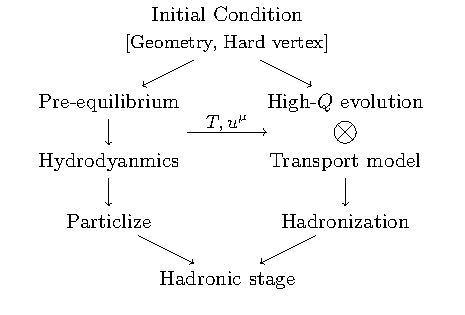
\includegraphics[width=.8\textwidth]{flowchart.pdf}
\caption{hh}
\label{fig:flowchart}
\end{figure}

In the previous two chapters, we have introduced the left branch of this flow chart, which is a relativistic viscous hydrodynamics based simulation for the bulk medium evolution.
The right branch is a model for the hard parton (heavy flavor) evolution.
The heavy quarks are produced in hard processes.
The hard processes contains both the hard matrix-element as well as the virtuality evolution of the parton (the DGLAP evolution or termed vacuum-like evolution).
One complication in the presence of medium, one complication is that vacuum-like evolution starts to occupied the same space-time of the medium induced processes at low-virtuality.
And should one interfaces the two calculations is still an interesting topic under debate.
One of the many obstacles is that multiple emissions / branchings are treated very differently in the two calculations.
For the vacuum-like evolution, the evolution variable is the virtuality scale with the space-time information integrated out, while the transport model evolves the systems in time, with virtuality integrated out below a certain scale.
There are many recent progress in both theory developments and newly design event-generators to solve this problem.
In this chapter, we shall focus on one possible solution to interface the two in section 1.
The in medium propagation of parton requires the medium properties as input. 
To zeros order of approximation, we specify the medium with its flow velocity and the equilibrium temperature, although the viscous hydro provides far more off-equilibrium information. 
This is discussed in section 2.
The heavy flavor hadronization model is introduced in section 3, which is a previously developed model that interpolates high-$p_T$ fragmentation processes and low-$p_T$ in medium recombination production of heavy hadrons.
Finally, in section 4, we also briefly introduced how this simulation framework of open heavy flavor can be coupled to the quarkonium evolution, but for more details, please refers to the thesis work [].

\section{Coupling transport dynamics to initial production}
The initial hard processes are computed using perturbative QCD based or related Monte-Carlo event generator.
The general set up for such a computation in proton-proton collision is the factorization theorem \ref{fig:factorization}.
Where the perturbative QCD calculation provides the physics at short distance (a hard scale $Q^2$): the partonic matrix-elements $\hat{\sigma}_{ij\rightarrow kl}$.
The partonic configuration inside the proton characterized by the parton-distribution function (PDF) and the hadronization of the final state parton into hadrons are non-perturbative inputs.
Although these non-perturbative objects general cannot be computed from first principal and has to be extracted from measurements, their scale evolution in $Q^2$ can be described in perturbative QCD, knowns as the DGLAP evolution equations.
This scale dependence comes from that the exclusive process  $i+j \rightarrow k+l$ described by the fixed order matrix-elements is always modified by the parton branching and virtual correction that is of order $\alpha_s \ln Q^2/\mu^2$.
These corrections takes into account the fact that the initial high-virtuality parton $i$ (or $j$) may also come from a splitting processes of low virtuality parton $i'$ (or $j'$) from the proton, including virtually correction. 
Similarly, the final state high virtuality parton $k$ (or $l$) may also splits into a low virtuality parton $k'$ (or $l'$) before it becomes a hadron, including virtual correction.
The same argument also applies to partons $i', j', k', l'$. 
Eventually, one gets a series of contribution where although each term contains an additional power of $\alpha_s$, but is magnified by $\ln Q^2/\mu^2$ if there is a large gap between the hard scale $Q^2$ and the PDF scale $\mu^2$ at which it is measured.
The DGLAP evolution equations resum these logarithmic contributions systematically to increase the predictive power of the perturbative calculation of the inclusive cross-section.
Moreover, a useful parton-shower picture can be built from the process and with a probabilistic interpretation and Monte Carlo technique, one can mimic the exclusive final states from these sequences of parton branching processes.

In our studies, we have tried to use both inclusive cross-section program as well as Monte-Carlo event generator to initialize the heavy quark production.
Next we will explain their merits and draw backs for our purposes.

\paragraph{Initialize from inclusive cross-section program}
We use FONLL (Fixed Order Next to Leading Log) to generate the inclusive production cross-section of heavy flavor at partonic level.
The FONLL program is a combination of the fixed order (NLO) massive matrix-elements and a massless resummation program.
It predicts the single inclusive differential cross-section $d^2\sigma/dydp_T$. 
Then, one can sample the initial heavy quark's momentum from this differential cross-section.
The advantages are
\begin{itemize}
\item[1.] Sampling / weighting the inclusive cross-section is fast.
\item[2.] Provide interface to nuclear PDFs.
\item[3.] Goes back to NLO accurate cross-section at low $p_T$.
\end{itemize} 
However, there are also disadvantages, 
\begin{itemize}
\item[1.] It only predicts single particle distribution and one cannot initialize the correlation of the $Q-\bar{Q}$ pair. This is not a problem for open heavy flavor observables, but would be a problem for quarkonium study.
\item[2.] The space-time picture of the production process is lost. One do not know whether the virtuality evolution takes a finite amount of time. So we have to assume charms quarks are produced at proper time $t=0^{+}$, which is always before the in-medium transport. But later we will see that from event generator simulations, the evolution can take a finite amount of time, overlapping with the QGP evolution.
\item[3.] Lacking the exclusive final state. Again, it is not a problem for open-heavy flavor study. But to describe full jets, one really needs an exclusive partonic final state of the virtuality evolution to initilize the partonic transport model.
\end{itemize}


\paragraph{Initialize from Monte-Carlo event generator.}

\begin{figure}
\centering
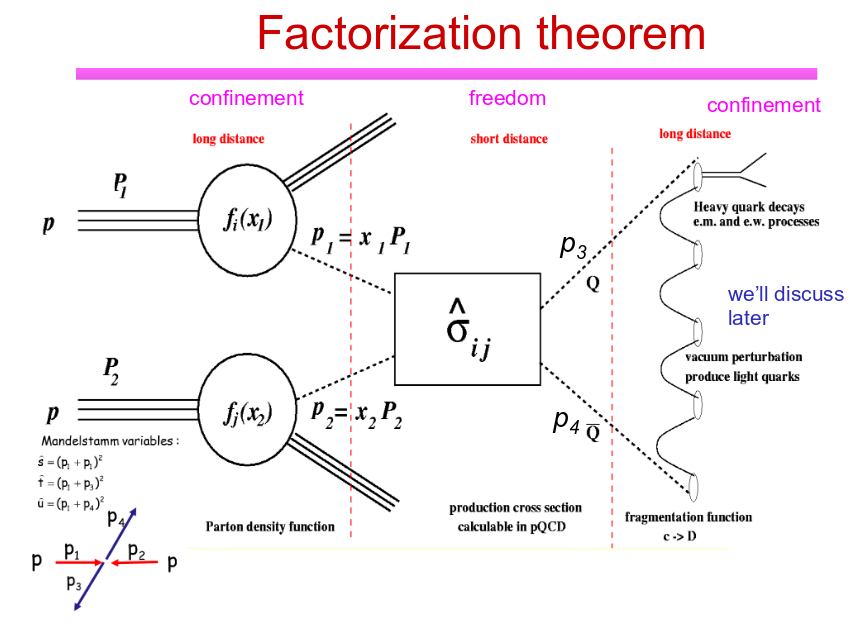
\includegraphics[width=\textwidth]{factorization.png}
\caption{
%https://indico.cern.ch/event/680421/contributions/3096162/attachments/1697092/2731944/J.Huston_Introduction_to_QCD_from_an_LHC_perspective-02.pdf
}
\label{fig:factorization}
\end{figure}


\section{Coupling transport dynamics to an evolving medium}

\section{Heavy-flavor hadronization and hadronic stage}

\section{Coupling open-heavy flavor to quarkonium evolution}
